% !TeX spellcheck = cs_CZ
%{\tikzset{external/prefix={tikz/MAI/}}
% \tikzset{external/figure name/.add={ch05_}{}}
%---------------------------------------------------------------------------------------------------
% file: Differential_Calculus_applications.tex
%---------------------------------------------------------------------------------------------------
\setchaptertoc
\chapter{Aplikace diferenciálního počtu}\label{mai:IchapVI}

%================Kapitola: Analýza průběhu funkce ==================================================
\section{Analýza průběhu funkce}\label{mai:IchapVIsecI}
  Diferenciální počet má rozsáhlou oblast užití. V této kapitole ukážeme použití výsledků
  předchozích kapitol k vyšetřování průběhu funkce a vlastnosti rovinných křivek. Pomocí derivace
  můžeme studovat vlastnosti funkce, které usnadní vyšetřování jejího průběhu. 

  Jednou z důležitých vlastností funkce je její \uv{monotonie}, kterou jsme definovali již v odst.
  \ref{mai:IchapIIIsecIssecIII} kap. \ref{mai:IchapIII}. Proto je při vyšetřování průběhu
  funkce důležité určit množiny (často jsou to intervaly), na nichž je funkce monotónní, jinak
  řečeno, najít \uv{intervaly monotonie funkce} (viz
  \cite[s.~208]{Brabec1989}). 
    \begin{enumerate}[noitemsep]
      \item Zjistíme \textbf{definiční obor funkce}, vyjádříme jej v intervalech a z nich poznáme,
        kde je funkce \textbf{spojitá}. Funkce je spojitá v $(a,b)$ pro každý bod tohoto intervalu,
        když $\abs{f(x)-f(c)}<\varepsilon$, kde $\varepsilon>0$ je libovolně zvolené číslo, a pro
        všechna \(x\) z okolí bodu $c$ je $\abs{x-c}<\delta$, kde $\delta>0$ je na $\varepsilon$
        nezávislé.
      \item Určíme, je-li funkce \textbf{lichá} $f(-x)=-f(x)$ nebo \textbf{sudá} $f(-x)=f(x)$. Je-li
        funkce lichá, je souměrná podle středu souměrnosti (obyčejně to bývá počátek souřadnic
        $xy$), je-li sudá, je souměrná podle osy \(y\).
      \item Určíme \emph{průsečíky křivky s osami pravoúhlých souřadnic}. Body, ve kte\-rých křivka
        protíná osu \(x\) spolu s body, ve kte\-rých není křivka spojitá, rozlišují intervaly, v nichž
        je graf křivky nad osou \(x\) od intervalů, ve kterých je graf křivky pod osou \(x\).
      \item V krajních bodech definičních intervalů, ve kterých je funkce spojitá, stano\-víme
      \emph{limity funkce} a dále $$\lim_{x \to \pm \infty}f(x).$$
      \item Vypočítáme $f'(x)$ a $f''(x)$, abychom zjistily, kde je funkce \emph{rostoucí}     
        $f'(x)>0$, \emph{klesající} $f'(x)<0$ a kde jsou \emph{lokální extrémy}. Dostaneme-li
        dosazením kořenů rovnice $f'(x)=0$ do $f''(x)$ hodnotu $f''(x)>0$, má funkce lokální
        minimum, při $f''(x)<0$ má funkce lokální maximum. V intervalech, kde $f''(x)>0$, je křivka
        \textbf{konvexní (vypuklá)}, kde $f''(x)<0$, je křivka \textbf{konkávní (vydutá)}. Body, v
        nichž $f''(x)$ mění znaménko, jsou \textbf{inflexní body}. Najdeme je tak, že stanovíme
        hodnoty \(x\), pro které je $f''(x)=0$ nebo neexistuje. Číslo $c$ je inflexní bod, když
        existuje takové okolí bodu $c$, že pro $x>c$ je oblouk křivky konvexní a pro $x<c$ konkávní.
        Je nutné si uvědomit, že když má $f'(x)$ konečnou derivaci, je inflexní bod $c$ taky nulovým
        bodem druhé derivace čili kořenem rovnice $f''(x)=0$. Obrácená věta neplatí, tj. z
        $f''(x)=0$ nevyplývá, že v bodě $c$ má $f'(x)$ extrém a že bod $c$ je inflexním bodem.
      \item \textbf{Asymptota} je tečna křivky \(f(x)\), jejíž bod dotyku je v nekonečnu. Platí-li  
        $$\lim_{x \to a}f(x) =  \pm\infty,$$ je přímka $x=a$ její asymptotou. Jinak asymptoty mají
        rovnici $y=kx+q$, kde \(x\) a \(y\) jsou souřadnice bodů na asymptotách. Existují-li konečné
        limity $$\lim_{x \to \pm\infty}\frac{f(x)}{x}=k$$  a $$\lim_{x \to \pm\infty}[f(x)-kx] =q$$
        pak je asymptotou přímka $y=kx+q$. Můžeme-li rovnici křivky rozložit (tj. rozložit její
        pravou stranu, oby\-čejně dělením čitatele jmenovatelem, má-li tvar zlomku) na dvě části, z
        nichž jedna má tvar $kx+q$ a druhá zbytek $\varphi(x)$, tj. $f(x)=kx+q+\varphi(x)$ a
        $\varphi(x)_{x\rightarrow \pm\infty}\rightarrow 0$, je přímka $y=kx+q$ asymptotou.
      \item Zpřesnění grafu křivky provedeme sestavením tabulky souřadnic dalších bodů křivky, tj.
        ke zvoleným hodnotám \(x\) (z definičního oboru funkce) vypočítáme hodnoty \(y\). Do dalších
        řádků tabulky zapíšeme hodnoty  $f'(x)$ a $f''(x)$, ve kterých intervalech je funkce
        \emph{rostoucí}, ve kterých \emph{klesá}, kde je \emph{vypuklá}, kde je \emph{dutá}, kde
        jsou \emph{lokální extrémy}, \emph{inflexní body} apod., případně sestavíme dílčí tabulky
        pro jednotlivé \emph{charakteristické vlastnosti} vyšetřované funkce.
    \end{enumerate}
    %-------------------- EXAM001 --------------------------------------
    % !TeX spellcheck = cs_CZ
\begin{mathexam}{Vyšetřete průběh funkce \(f(x):y=\frac{1+x^2}{1-x^2}\)}{exam003}
  \begin{enumerate}[noitemsep]
    \item Definiční obor $D_f=\realset-\{±1\}=(-\infty,-1)\cup(-1,1)\cup(1,+\infty)$
    \item Funkce je sudá $$f(-x)=f(x): \frac{1+x^2}{1-x^2}=\frac{1+(-x)^2}{1-(-x)^2}.$$ Funkce není
        periodická.
    \item Stanovíme funkční hodnoty v krajních bodech definičního obor $1, -1$ a v nevlastních
        bodech $-\infty,+\infty$.Protože je funkce \textbf{sudá}, omezíme se jen na vyšetřování
        nezáporné části. Nejprve vlastnosti funkce v okolí bodu $1$. Ten nepatří do $D_f$ a proto
        určíme limity funkce v pravém a levém okolí tohoto bodu. $$\lim_{x\to
        1_{-}}=\frac{1+x^2}{1-x^2}.$$ Pro výpočet limity použijeme substituci $y=1-x^2$: 
        $$\lim_{y\to0+}\frac{2-y}{y}=+\infty$$ \footnote{$\lim_{x\to0_+}\frac{1}{x}=\infty$} proto
        
        $$\lim_{x\to1_{-}}\frac{1+x^2}{1-x^2}=+\infty.$$ Obdobně dojdeme k
        $$\lim_{x\to1_+}\frac{1+x^2}{1-x^2}=-\infty.$$ A konečně v nevlastních bodech $±\infty$ je
        limita $$\lim_{x\to±\infty}\frac{1+x^2}{1-x^2} = \lim_{x\to\pm\infty}\frac{1}{1-x^2} +
        \lim_{x\to\pm\infty}\frac{x^2}{1-x^2}=0-1=-1.$$ Výpočtem limit jsme zároveň určili dva
        absolutní (globální) extrémy a jeden lokální:
        \begin{itemize}
          \item v intervalu $(-1,1)$ má funkce maximum $\infty$ a minimum $1$,
          \item v intervalech $(-1,1)\cup(1,+\infty)$ má funkce minimum $-\infty$ a maximum $-1$.
        \end{itemize}
    \item Nyní vyšetříme zda, případně kolik a jaké, má funkce $f(x)$ průsečíky s osami souřadnic. S
        osou $x$ nemá funkce žádné průsečíky, protože pro $y=0$ není definována
        $H_f=\realset-\{-1,1\rangle$. Pro $x=0$ je $y=\frac{1+0^2}{1-0^2}=1$, proto má $f(x)$ právě
        jeden průsečík s osou $y$ a to $[0,1]$.
    \item Zatím jsme zjistili, že naše funkce není definována v bodech $1$ a $-1$ a proto není
        spojitá v  $\realset$. Nevíme však, jaký je její průběh v jednotlivých intervalech
        definičního oboru.  Abychom získali názornější představu o průběhu funkce, zjistíme má-li
        derivaci.
        \begin{align*}
          y' &= \frac{(1+x^2)'(1-x^2 )-(1+x^2)(1-x^2 )'}{(1-x^2)^2} \\
          y' &= \frac{2x(1-x^2 )-(1+x^2 )(-2x)}{(1-x^2 )^2}         \\
          y' &= \frac{4x}{(1-x^2 )^2}
        \end{align*}
        Protože má vlastní derivaci\footnote{$f(x)$ je spojitá v intervalech $(-\infty,-1),
        (-1,1),(1,\infty)$  věta s spojité funkci}, můžeme určit její vlastnosti v intervalech
        $\langle0,1)$ a $(1,\infty)$. V těchto intervalech je $y'>0$ a proto jde o funkci ryze
        monotónní, rostoucí \footnote{Plyne z věty o postačujících podmínkách ryzí monotónnosti
        funkce na intervalu} v daných intervalech \footnote{V intervalech
        $(-\infty,-1),(-1,0\rangle$ je funkce klesající.}. Výpočtem zjistíme druhou derivaci funkce.
        Ta nám pomůže určit další extrém v intervalu $\langle0,1)$ a zároveň vyšetřit
        \textbf{konkávnost} a \textbf{konvexnost}.
        \begin{align*}
          y'' &= \frac{(4x)' (1-x^2 )^2-(4x)(1-2x^2+x^4 )'}{(1-x^2 )^4}  \\
          y'' &= \frac{4(1-2x^2+x^4 )-4x(-4x+4x^3 )}{(1-x^2 )^4}         \\
          y'' &= \frac{4(1-x^2 )(3x^2+1)}{(1-x^2 )^4}                    \\
          y'' &= \frac{4(3x^2+1)}{(1-x^2 )^3}
        \end{align*}
        Abychom mohli určit lokální extrém funkce $f(x)$ v intervalu $\langle0,1)$, pomocí druhé
        derivace, musíme najít kořeny rovnice $f' (x)=0$. V našem případě
        $$y'=\frac{4x}{(1-x^2)^2}\Rightarrow\frac{4x}{(1-x^2)^2}=0\rightarrow x_0=0,$$ tento kořen
        \footnote{stacionární bod}  pak dosadíme do druhé derivace, tj. 
        $$y''(0)=\frac{4(3\cdot0^2+1)}{(1-0^2 )^3}=4,$$ protože je $f''(x)>0$, má v bodě $x_0$
        lokální minimum. Můžeme rovněž konstatovat, že funkce nemá inflexní body \footnote{Pro
        existenci inflexního bodu je nutné splnění jedné z podmínek a to buď $f''(x_0)=0$, nebo
        $f''(x_0)$ neexistuje.}. Konkávnost a konvexnost funkce v intervalech $\langle0,1)$ a
        $(1,\infty)$ vyšetříme pomocí vlastností druhé derivace funkce. Tedy
        \begin{itemize}
          \item $\langle0,1): y''=\frac{4(3x^2+1)}{(1-x^2 )^3} >0 \Rightarrow$ funkce je v tomto
                intervalu \textbf{konvexní},
          \item $(1,\infty): y''=\frac{4(3x^2+1)}{(1-x^2 )^3} <0 \Rightarrow$ funkce je v tomto
                intervalu \textbf{konkáv\-ní}.
        \end{itemize}
    \item Z předchozích výpočtů plyne, že křivka má asymptoty $y=-1,x=\pm1$.
  \end{enumerate}
  {\centering \captionsetup{type=figure}          % %\ref{MAI:fig_028}
    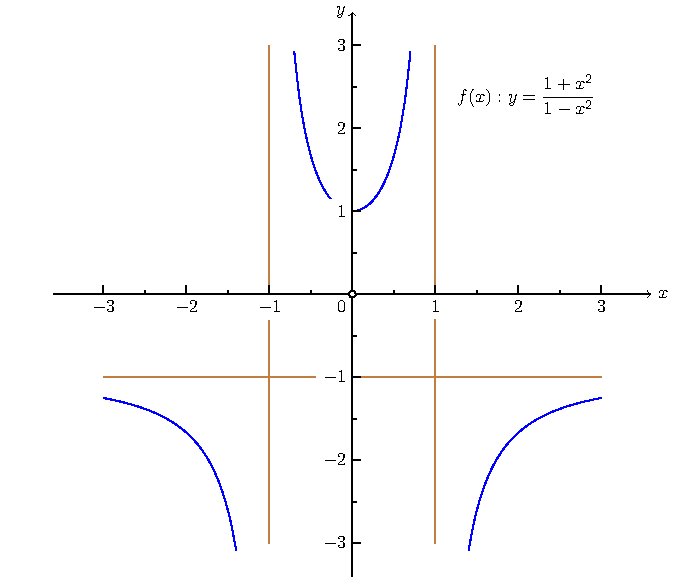
\includegraphics[width=1\linewidth]{mai_fig028.pdf}
    \captionof{figure}{Graf funkce $f(x):y=\dfrac{1+x^2}{1-x^2}$}
    \label{MAI:fig_028}
  \par}
\end{mathexam}  
    %-------------------------------------------------------------------

%================Kapitola: Aplikace diferenciálního počtu =========================================
\twocolumn[\section{Fyzikální a jiné aplikace derivace}\label{mai:IchapVIsecII}]
    V předcházející kapitole \ref{mai:IchapVIsecI} jsou uvedeny jednoduché příklady na užití první a
    druhé derivace. V této kapitole jsou soustředěny slovní úlohy na maxima a minima z různých
    oborů.
    %--------------------------------------------------------------
    % !TeX spellcheck = cs_CZ
\begin{mathexam}{Je dán trojúhelník s vrcholy \(A[0, 0]\), \(B[4, 0]\), \(C[1, 3]\). Mezi všemi
  obdélníky vepsanými danému trojúhelníku, se stranou („základnou“) \(z\) ve straně \(c\) (označení
  viz obr. \ref{mai:fig062}), máme najít ten, který má maximální obsah.}{exam092}

  {\centering
    \captionsetup{type=figure}
    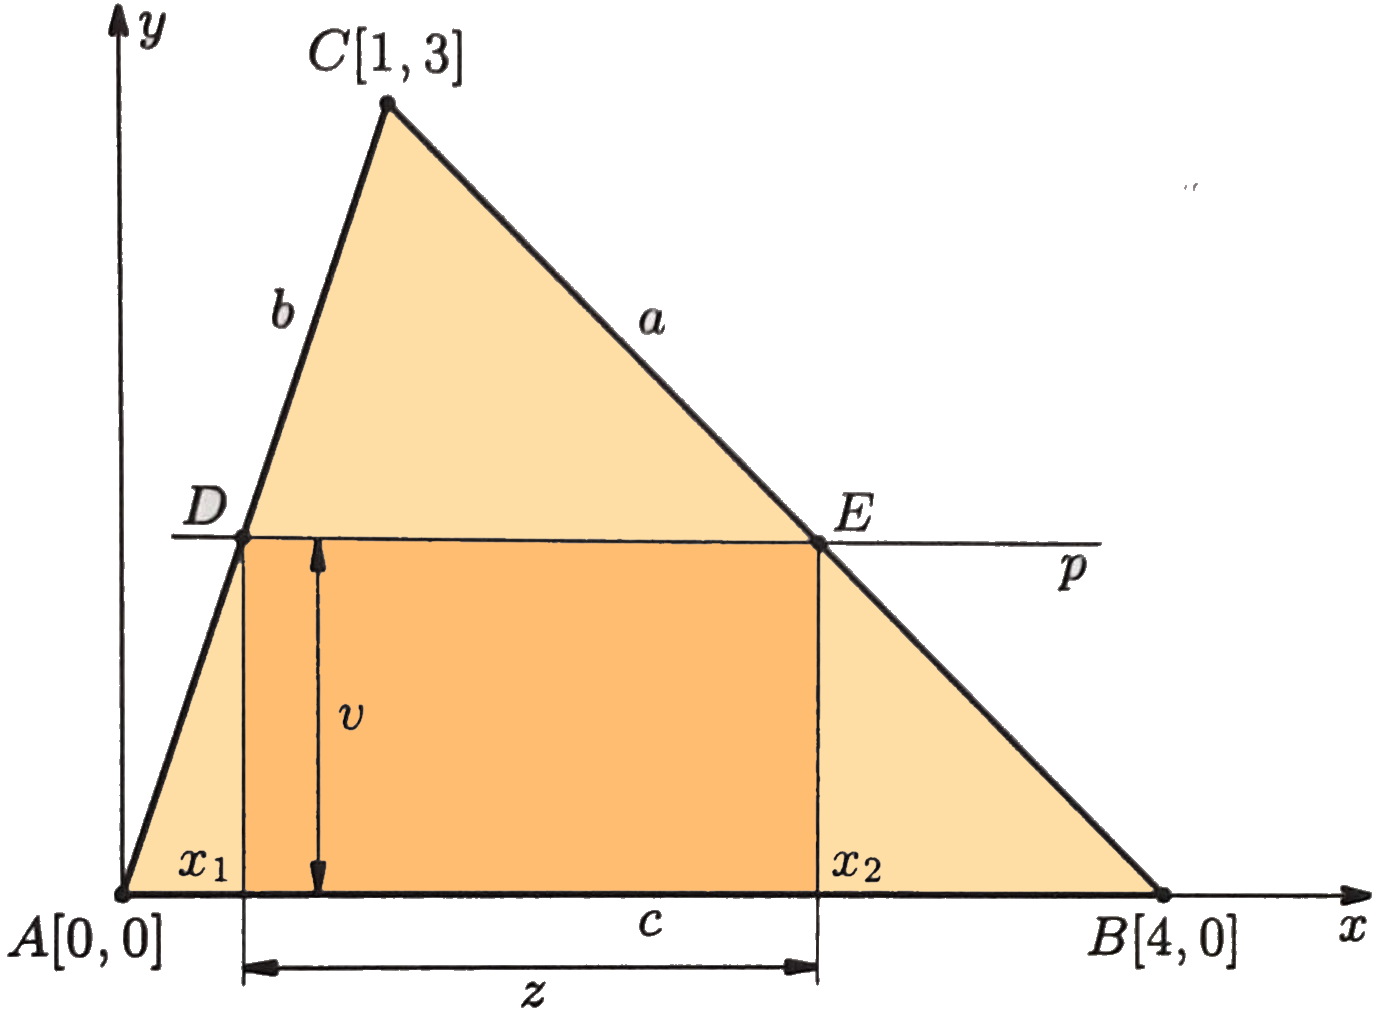
\includegraphics[width=1\linewidth]{mai_fig062.png} 
    \captionof{figure}{K příkladu \ref{mai:exam092}. Kredit: \cite[s.~46]{rektorys2011}}
    \label{mai:fig062}
  \par}
  
  Napišme nejprve rovnice stran \(a\), \(b\). Strana \(b\) (přesněji: přímka obsahující stranu
  \(b\)) má zřejmě rovnici
  \begin{equation*}
    y = 3x
  \end{equation*}
  Přímka, v níž leží strana \(a\), má směrnici
  \begin{equation*}
    k = \dfrac{3-0}{1-4} = -1,
  \end{equation*}
  a tedy podle rovnice \(y-y_0 = k(x-x_0)\) dostáváme 
  \begin{equation*}
    y - 0 = -1\cdot(x - 4) \quad\Rightarrow\quad y = -x + 4.  
  \end{equation*}
  Pro obsah \(S\) vepsaného obdélníka platí podle označení v obr. \ref{mai:fig062} 
  \begin{equation*}
    S = zv.
  \end{equation*}
  Za proměnnou zde bude výhodné volit „výšku“ \(v\). „Základnu“ \(z\) pak vypočteme (viz obr.
  \ref{mai:fig062}) jako rozdíl
  \begin{equation}\label{mai:eq087}
    z = x_2 - x_1,
  \end{equation}
  kde \(x_1\), resp. \(x_2\) je souřadnice \(x\) průsečíku přímky \(y = v\) (přímka \(p\) na obr.
  \ref{mai:fig062}) se stranou \(b\), resp. \(a\). Rovnice těchto stran jsou dány vztahy \(y = 3x\)
  a \(y = -x + 4\). Dosadíme-li podle \(y = v\rightarrow\)  \(v\) za \(y\) do těchto rovnic,
  dostaneme právě \(x_1\) a \(x_2\). Bude
  \begin{equation*}
    v = 3x_1, \qquad v = -x_2 + 4,
  \end{equation*}
  odkud (při zvoleném \(v\)) plyne
  \begin{equation*}
    x_1 = \dfrac{v}{3}, \qquad  x_2 = 4 - v 
  \end{equation*}
  a podle \ref{mai:eq087}
  \begin{equation*}
    z = x_2 - x_1 =  4 - \dfrac{4}{3}v
  \end{equation*}
  a konečně pro obsah vepsaného obdélníku dostáváme jednoduchou rovnici
  \begin{equation}\label{mai:eq088}
    S = zv = \left(4 - \dfrac{4}{3}v\right)v = 4v - \dfrac{4}{3}v^2.
  \end{equation} 
  Tím je obsah \(S\) obdélníka daný jako funkce zvolené výšky \(v\). Zvolíme-li například \(v=1\),
  bude obsah \(S\) obdélníka z obr. \ref{mai:fig062} roven číslu \(4\cdot1 - \frac{4}{3}\cdot1^2\). 
  
  Budeme hledat (absolutní) maximum funkce (\ref{mai:eq088}) na intervalu \(\langle0,3\rangle\)
  (neboť nemůžeme zvolit \(v\) větší než 3). Ale pro \(v=0\) a \(v=3\) je \(S=0\) a všude jinde je
  \(S > 0\), takže budeme hledat lokální maximum funkce (\ref{mai:eq088}) na otevřeném intervalu
  \((0,3)\). Derivováním (\ref{mai:eq088}) podle proměnné \(v\) však máme
  \begin{equation*}
    S' = 4 - \dfrac{8}{3}v, \qquad S'' = -\dfrac{8}{3}.
  \end{equation*}
  Položíme-li nyní pravou stranu rovnu nule, dostaneme 
  \begin{equation*}
    4 - \dfrac{8}{3}v = 0 \quad\Rightarrow\quad v = \dfrac{12}{8} = \dfrac{3}{2}.
  \end{equation*}
  Přitom podle druhé derivace obsahu je všude, a tedy i v bodě \(\frac{3}{2}\), je
  \(S''=-\frac{8}{3}<0\) takže v bodě \(v = \frac{2}{3}\) je ostré lokální maximum. Zároveň pro
  \(v=\frac{3}{2}\) bude
  \begin{equation*}
    z = 4 - \dfrac{4}{3}\cdot\dfrac{3}{2} = 2.
  \end{equation*}
  Hledaný obdélník maximálního obsahu bude mít rozměry: \(z = 2\), \(v = \frac{3}{2}\), a tedy obsah
  \(S = 3\).    
\end{mathexam}
    %--------------------------------------------------------------
    %--------------------------------------------------------------
    % !TeX spellcheck = cs_CZ
\begin{mathexam}{Z břevna kruhového průřezu s poloměrem \(r = \protect\SI{20}{\protect\cm}\) máme
  vytesat trám, který bude mít průřez ve tvaru obdélníka se stranami \(z\) a \(v\) („základnou“ a
  „výškou“). Jak máme volit \(z\) a \(v\), aby trám měl maximální nosnost, víme-li, že jeho nosnost
  je úměrná první mocnibibeně \(z\) a druhé mocnině \(v\)?}{exam091}
   
  {\centering
    \captionsetup{type=figure}
    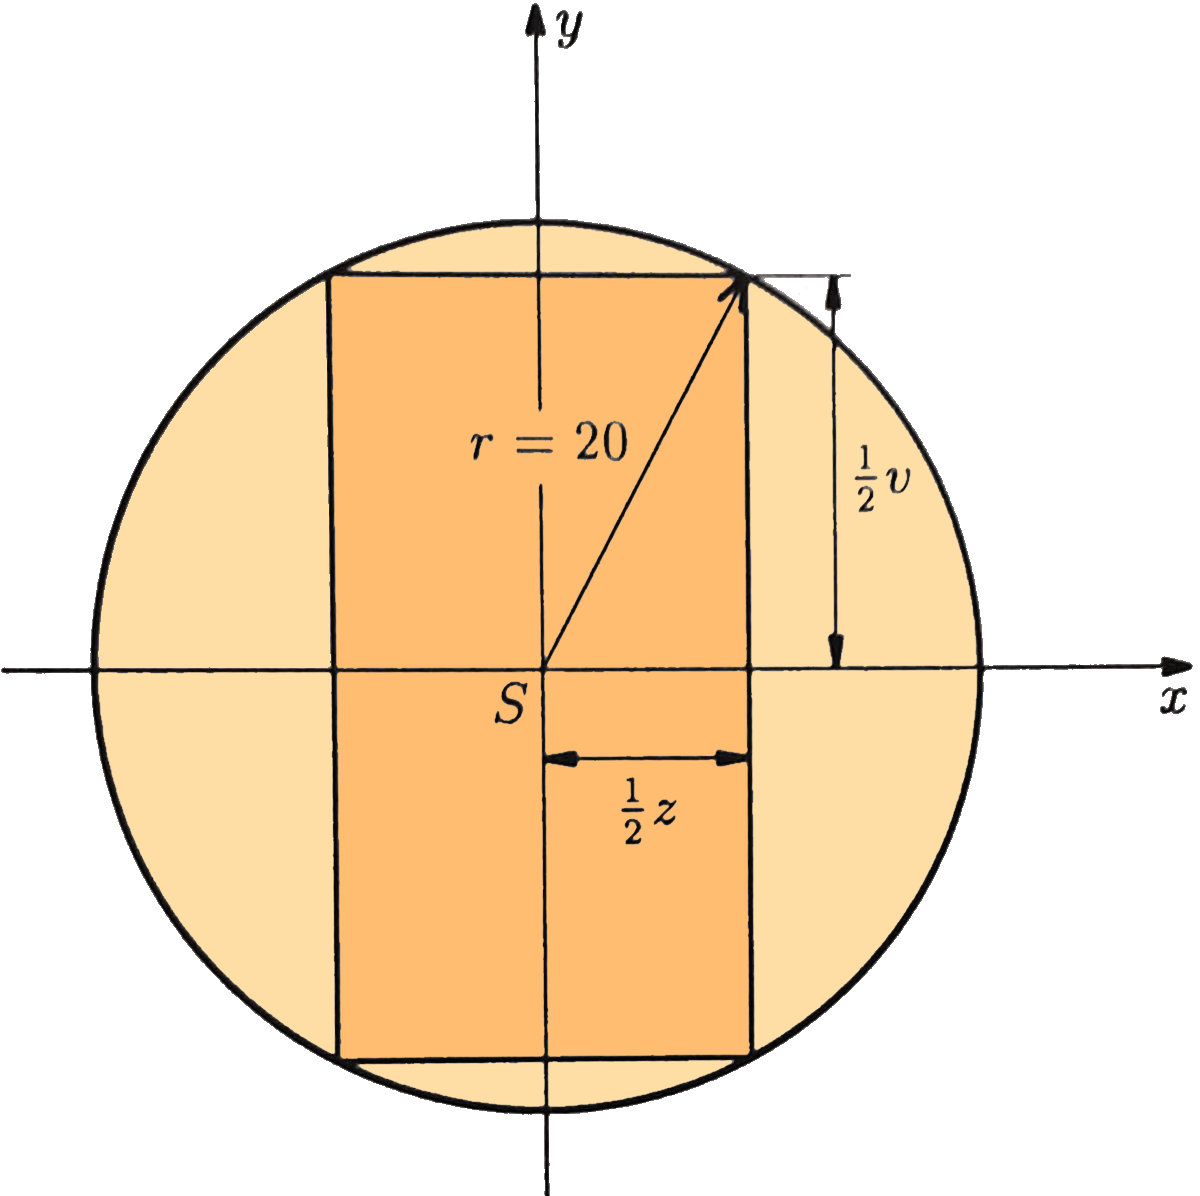
\includegraphics[width=1\linewidth]{mai_fig061.png} 
    \captionof{figure}{K příkladu \ref{mai:exam091}. Kredit: \cite[s.~47]{rektorys2011}}
    \label{mai:fig061}
  \par}
  
  Matematická formulace: Jaké rozměry má mít obdélník vepsaný do kružnice s poIoměrem \SI{20}{\cm},
  má-li být součin základny \(z\) a druhé mocniny výšky v maximální,
  \begin{equation*}
    y = z\cdot v^2 = ?
  \end{equation*}
  Zvolme za proměnnou z. Podle Pythagorovy věty platí (viz \ref{mai:fig061})
  \begin{equation*}
      r^2 = \left(\dfrac{z}{2}\right)^2 + \left(\dfrac{v}{2}\right)^2,
  \end{equation*}
  odkud 
  \begin{equation*}
      v^2 = 4r^2 - z^2.
  \end{equation*}
  Máme tedy najít maximum funkce
  \begin{equation}\label{mai:eq086}
      y = zv^2 = z(4r^2 - z^2) = 4r^2z - z^3,
  \end{equation}
  a to na intervalu \((0,40)\), neboť \(z\) nemůže být větší než \(2r = 40\). Ale funkce
  (\ref{mai:eq086}) je na tomto intervalu nezáporná a pro \(z = 0\) a \(z = 40\) je rovna nule
  (neboť pak \(4r^2 - z^2 = 0\). Hledáme tedy lokální maximum funkce (\ref{mai:eq086}) v otevřeném
  intervalu \(0,40)\). 

  Funkce (\ref{mai:eq086}) má všude první a druhou derivaci,
  \begin{equation*}
      y' = 4r^2 - 3z^2, \qquad\qquad y'' = -6z.
  \end{equation*}
  Může tedy předně nabývat v intervalu \((0, 40)\) lokálního extrému jen tam, kde je \(y'=0\), tj.
  kde
  \begin{equation*}
      4r^2 - 3z^2 = 0.
  \end{equation*}
  Odtud plyne, neboť má být \(z > 0\), že
  \begin{equation*}
      z = \sqrt{\dfrac{4r^2}{3}} = \dfrac{2}{\sqrt{3}}r = \dfrac{2\sqrt{3}}{3}r = 
          \dfrac{2\sqrt{3}}{3}20 \simeq \num{23.1}.
  \end{equation*}
  Pro \(v\) pak \(z\) dostaneme
  \begin{equation*}
      v = \sqrt{4r^2 - \dfrac{4}{3}r^2} = \sqrt{\frac{8}{3}\cdot20^2}\simeq\num{32.6}
  \end{equation*}
  V bodě \(z = \num{23.1}\) bude mít funkce (\ref{mai:eq086}) skutečně lokální maximum, a to ostré,
  neboť druhá derivace je v tomto bodě záporná.
\end{mathexam}
    %--------------------------------------------------------------
    %--------------------------------------------------------------
    % !TeX spellcheck = cs_CZ 
\begin{mathexam}{Světelný zdroj \(B\) (např. pouliční svítilna) má vzdálenost \qty{36}{\m} od
  světelného zdroje \(A\). Zdroj \(B\) má osmkrát větší intenzitu než zdroj \(A\). Který bod na
  spojnici obou zdrojů bude nejméně osvětlený? (Přitom intenzita osvětlení světelným zdrojem je
  přímo úměrná intenzitě zdroje a klesá s druhou mocninou vzdálenosti od uvažovaného
  zdroje.)}{exam093} 
  
  {\centering
    \captionsetup{type=figure}
    \luafigure[1]{mai_fig063.png} 
    \captionof{figure}{K příkladu \ref{mai:exam093}. Kredit: \cite[s.~48]{rektorys2011}}
    \label{mai:fig063}
  \par}      

  Matematická formulace: Označme \(a\) intenzitu zdroje \(A\). Pak intenzita zdrojo \(8\) je \(8a\).
  Označme dále \(x\) vzdálenost bodu \(P\) na spojnici bodů \(A\) a \(B\) meřenou od zdroje \(A\).
  Pak intenzita osvětlení v bodě \(P\) od zdroje \(A\) bude úměrná číslu \(\frac{a}{x^2}\) zdroje B
  číslu \(\frac{8a}{(36 - x)^2}\) (se stejnou konstantou úměrnosti). Máme tedy najít v intervalu
  \((0,36)\) takové \(x\), pro které bude součet obou intenzit minimalni, a tj.
  \begin{equation}\label{mai:eq089}
    y = \dfrac{a}{x^2} + \dfrac{8a}{(36 - x)^2} = \text{min}
  \end{equation}
  Ale funkce \ref{mai:eq089} má všude v otevřeném intervalu  \((0,36)\) první a druhou derivaci.
  Nastává chvíle si procvičit derivování podílu:
  \begin{gather*}
    \begin{align*} 
      \left(\dfrac{a}{x^2}\right)'          
        &= (ax^{-2})' = -\dfrac{2a}{x^3},   \\ 
      \left( \dfrac{8a}{(36 - x)^2}\right)' 
        &= \dfrac{(8a)'\cdot(36 - x)^2 - (8a)\cdot(36^2 - 72x + x^2)'}{(36 - x)^4} \\
        &= \dfrac{-8a(-72 + 2x)}{(36 - x)^4} 
         = +\dfrac{8a\cdot2\cdot\cancel{(36 - x)}}{(36 - x)^{\cancel{4}3}}
         =  \dfrac{16a}{(36 - x)^3}
    \end{align*}
  \end{gather*}
  (neboť \(8a = \text{konst}\), takže \((8a)' = 0\); k derivování funkce \(8a/(36 - x)^2\) jsme také
  mohli místo věty o derivování podílu použít větu o derivování složených funkcí a psát
  \begin{equation*}
    \dfrac{8a}{(36 - x)^2} = \dfrac{8a}{z}, \quad\text{kde}\quad z = 36 - x
  \end{equation*}  
  Tedy 
  \begin{align*}
    y'  &= -\dfrac{2a}{x^3} + \dfrac{16a}{(36 - x)^3} \\
    y'' &=  \dfrac{6a}{x^4} + \dfrac{48a}{(36 - x)^4}. 
  \end{align*}
  Jak víme, v bodě lokálního minima bude \(y' = 0\)
  \begin{equation}\label{mai:eq090}
    -\dfrac{2a}{x^3} + \dfrac{16a}{(36 - x)^3} = 0.
  \end{equation}
  Rovnici můžeme řešit tak, že zlomky na levé straně dáme na společného jmenovatele. (Zkuste to,
  nebude to hezká rovnice!) Ale má být \(x > 0\), \(36 - x > 0\), takže (\ref{mai:eq090}) můžeme
  zapsat ve tvaru
  \begin{align*}
    \dfrac{(36 - x)^3}{x^3} &= -\dfrac{16a}{2a} = 8 \qquad\text{takže}      \\
    \dfrac{36 - x}{x}       &= \sqrt[3]{8} \Rightarrow 36 - x = 2x.
  \end{align*}
  Zároveň \(y''>0\), takže v bodě \(x=12\) bude ostré lokální minimum. Nejméně osvětlený bod bude
  tedy ve vzdálenosti \qty{12}{\m} od zdroje \(A\).

  {\centering
  \captionsetup{type=figure}
  \luafigure[1]{mai_fig064.pdf} 
  \captionof{figure}{K příkladu \ref{mai:exam093}.}
  \label{mai:fig064}
  \par}   
\end{mathexam}
    %--------------------------------------------------------------